\documentclass{article}

\usepackage{arxiv}

\usepackage[utf8]{inputenc} % allow utf-8 input
\usepackage[T1]{fontenc}    % use 8-bit T1 fonts
\usepackage{lmodern}        % https://github.com/rstudio/rticles/issues/343
\usepackage{hyperref}       % hyperlinks
\usepackage{url}            % simple URL typesetting
\usepackage{booktabs}       % professional-quality tables
\usepackage{amsfonts}       % blackboard math symbols
\usepackage{nicefrac}       % compact symbols for 1/2, etc.
\usepackage{microtype}      % microtypography
\usepackage{graphicx}

\title{Exploring the EEG Signals of Schizophrenia}

\author{
    Maeve Samali
   \\
    School of Mathematics, Applied Mathematics \& Statistics \\
    University of Galway \\
  Galway, Ireland \\
  \texttt{\href{mailto:M.samali1@universityofgalway.ie}{\nolinkurl{M.samali1@universityofgalway.ie}}} \\
   \And
    Sarah Conway
   \\
    School of Mathematics, Applied Mathematics \& Statistics \\
    University of Galway \\
  Galway, Ireland \\
  \texttt{\href{mailto:S.Conway29@universityofgalway.ie}{\nolinkurl{S.Conway29@universityofgalway.ie}}} \\
   \And
    Hollie Keating
   \\
    School of Mathematics, Applied Mathematics \& Statistics \\
    University of Galway \\
  Galway, Ireland \\
  \texttt{\href{mailto:H.Keating3@universityofgalway.ie}{\nolinkurl{H.Keating3@universityofgalway.ie}}} \\
  }


% tightlist command for lists without linebreak
\providecommand{\tightlist}{%
  \setlength{\itemsep}{0pt}\setlength{\parskip}{0pt}}


% Pandoc citation processing
%From Pandoc 3.1.8
% definitions for citeproc citations
\NewDocumentCommand\citeproctext{}{}
\NewDocumentCommand\citeproc{mm}{%
  \begingroup\def\citeproctext{#2}\cite{#1}\endgroup}
\makeatletter
 % allow citations to break across lines
 \let\@cite@ofmt\@firstofone
 % avoid brackets around text for \cite:
 \def\@biblabel#1{}
 \def\@cite#1#2{{#1\if@tempswa , #2\fi}}
\makeatother
\newlength{\cslhangindent}
\setlength{\cslhangindent}{1.5em}
\newlength{\csllabelwidth}
\setlength{\csllabelwidth}{3em}
\newenvironment{CSLReferences}[2] % #1 hanging-indent, #2 entry-spacing
 {\begin{list}{}{%
  \setlength{\itemindent}{0pt}
  \setlength{\leftmargin}{0pt}
  \setlength{\parsep}{0pt}
  % turn on hanging indent if param 1 is 1
  \ifodd #1
   \setlength{\leftmargin}{\cslhangindent}
   \setlength{\itemindent}{-1\cslhangindent}
  \fi
  % set entry spacing
  \setlength{\itemsep}{#2\baselineskip}}}
 {\end{list}}
\usepackage{calc}
\newcommand{\CSLBlock}[1]{#1\hfill\break}
\newcommand{\CSLLeftMargin}[1]{\parbox[t]{\csllabelwidth}{#1}}
\newcommand{\CSLRightInline}[1]{\parbox[t]{\linewidth - \csllabelwidth}{#1}\break}
\newcommand{\CSLIndent}[1]{\hspace{\cslhangindent}#1}

\newcommand{\pandocbounded}[1]{#1}
\usepackage{booktabs}
\usepackage{longtable}
\usepackage{array}
\usepackage{multirow}
\usepackage{wrapfig}
\usepackage{float}
\usepackage{colortbl}
\usepackage{pdflscape}
\usepackage{tabu}
\usepackage{threeparttable}
\usepackage{threeparttablex}
\usepackage[normalem]{ulem}
\usepackage{makecell}
\usepackage{xcolor}
\begin{document}
\maketitle


\begin{abstract}
Enter the text of your abstract here.
\end{abstract}

\keywords{
    Electroencephelogram
   \and
    Schizophrenia
   \and
    Elastic Net
   \and
    Functional Data Analysis
  }

\section{Introduction}\label{introduction}

\label{sec:intro}

An electroencephalogram (EEG) is a non-invasive test used to measure
electrical activity in the brain by attaching 64 sensor nodes to the
scalp. Each sensor measures a single curve, so each test produces 64
curves. The data from EEG is commonly used to diagnose conditions such
as sleep disorders, seizures and schizophrenia

Schizophrenia is a mental health condition which is associated with
unusual activity in the frontal and prefrontal sections of the brain.

Sensory gating is the process by which the brain filters repeated,
expected or redundant stimuli. This process is impaired in individuals
with schizophrenia, particularly at the P50 (indicating pre-attentive
filtering of sensory information), N100 and P200 (both reflecting the
attention triggering/allocation process) regions of the EEG curve, which
occur 50, 100 and 200 ms after an auditory stimulus, respectively. The
impairment of the sensory gating process can be detected by a difference
in the amplitude of these deflections in the curve (Shen et al. 2020;
Boutros et al. 2009).

Functional data analysis (FDA) is a method of statistical analysis that
analyses each function as an individual sample, as opposed to
considering all the points along the curve separately. It is used when
the underlying curve is smooth and continuous (Ramsay and Silverman
2005). EEG curves are a type of functional data that indicates the
brain's electrical activity by the continuous flow of voltages over
time.

\begin{itemize}
\tightlist
\item
  Introduce EEG, how it relates to schizophrenia, and how FDA can be
  used to analyse curves
\item
  Current Literature - FDA for EEG signals or for schizophrenia has been
  used before? findings? etc.
\end{itemize}

\subsection{Data}\label{data}

Our data were taken from the National Institute of Mental Health (NIMH
project number R01MH058262), available from
\href{www.kaggle.com/datasets/broach/button-tone-sz/data}{Kaggle}

In our data, 40 subjects underwent three sensory conditions (25
controls, 15 cases) in which:

\begin{enumerate}
\def\labelenumi{\arabic{enumi}.}
\tightlist
\item
  Subjects press a button to immediately produce a sound
\item
  Subjects passively listen to the same sound without pressing a button
\item
  Subjects press a button, and no sound is produced.
\end{enumerate}

Each subject completed each of these sensory conditions up to 100 times.
Therefore, we have many repetitions of the same conditions for each of
the subjects. So in total we have approximately
\(64\times 40 \times 100 = 256,000\) curves.

\begin{itemize}
\tightlist
\item
  Explain the study background trials, conditions etc.
\end{itemize}

\section{Methods}\label{methods}

\label{sec:methods}

We used several methods: spline smoothing, permutation test, FPCA \&
mFPCA

\subsection{Smoothing}\label{smoothing}

Due to the inherently noisy nature of EEG signals, smoothing was applied
to the functional observations. When smoothing functions, it is
important to balance the trade-off between variance and bias. Variance
refers to the sensitivity of an estimated function to random
fluctuations in the observed data, while bias refers to systematic
deviation of the estimated function from the true underlying signal.
High variance may lead to overfitting and poor generalisability to new
data, whereas high bias may over smooth the data and obscure important
signal characteristics.

Spline smoothing was used to reduce noise while preserving the
underlying brain activity patterns. Specifically, 100 cubic B-spline
basis functions were defined over the domain of each EEG signal,
(0-1638ms). Using a relatively large number of basis functions provides
sufficient flexibility to represent complex functional features while
allowing smoothness to be controlled separately through penalisation.

A second-derivative roughness penalty was then applied. In penalised
smoothing approaches, smoothness is controlled by incorporating a
roughness penalty into the objective function used to fit the data,
rather than by restricting the number of basis functions available
(Ramsay and Silverman 2005). Penalising the second derivative
discourages rapid changes in curvature, allowing gradual variation in
the fitted function while reducing excessive wiggliness. In practice,
this encourages neighbouring B-spline coefficients to vary smoothly and
can be viewed as approximating penalties on finite differences between
adjacent coefficients. The roughness penalty pools information across
neighbouring regions of the function, resulting in more stable estimates
and reduced sensitivity to noise. Consequently, variance is reduced at
the cost of a small increase in bias, yielding smoother and more
interpretable functional representations of the EEG signals (Ramsay and
Silverman 2005; Gertheiss et al. 2024).

**insert plot of raw data and smoothed means

\begin{figure}[H]

{\centering 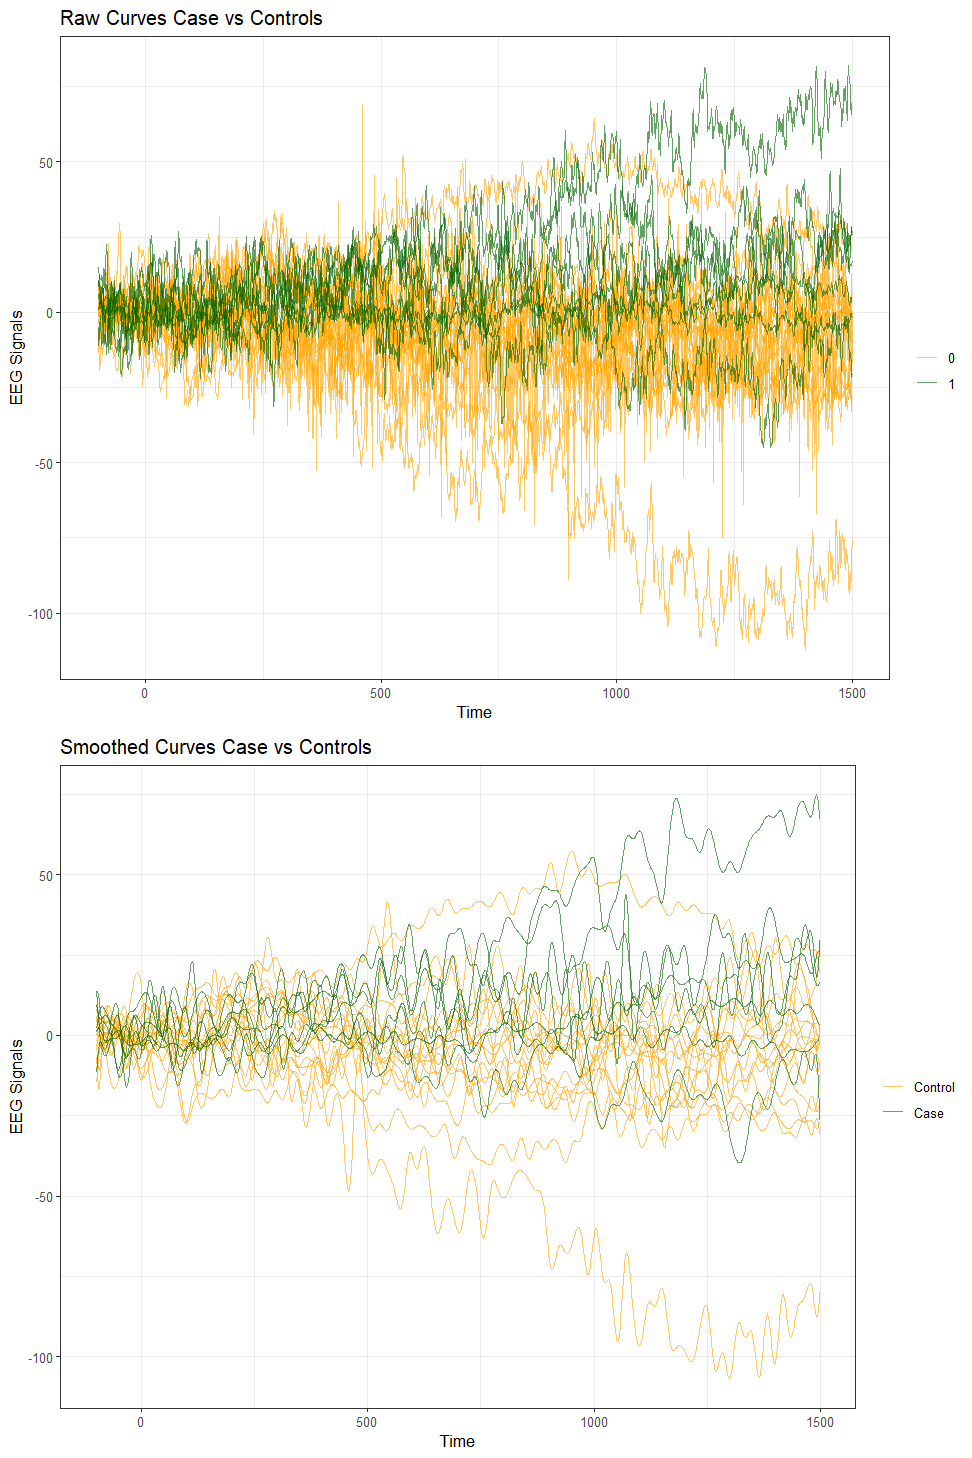
\includegraphics[width=0.8\linewidth]{Images/raw_smooth_data} 

}

\caption{Plots of raw and smoothed data, coloured by case-control status}\label{fig:unnamed-chunk-2}
\end{figure}

**insert formula

\subsection{Permutation test}\label{permutation-test}

Permutation t-tests were used to assess differences in functional EEG
trajectories between cases and controls. Permutation-based inference is
well suited to functional data and has been widely applied in the FDA
literature (Bugni and Horowitz 2021). The test evaluates the null
hypothesis that the mean functions of the two groups are equal across
the domain of the EEG signal.

Under the null hypothesis, group labels are exchangeable, meaning that
randomly reallocating observations between groups should not
systematically alter the value of the test statistic. The permutation
procedure repeatedly shuffles the case-control labels and recalculates
the test statistic for each permutation, generating an empirical null
distribution. The observed test statistic is then compared with this
distribution to determine statistical significance. The resulting
p-value represents the probability of obtaining a test statistic at
least as extreme as that observed if the null hypothesis were true.

When interpreting a permutation t-test plot for an a priori,
theory-driven hypothesis, statistical significance is indicated when the
observed test statistic exceeds the pointwise 0.05 critical value.
However, for post hoc, data-driven hypotheses, significance should be
assessed relative to the maximum 0.05 critical value, which controls for
multiple comparisons across the entire functional domain and provides
stronger control of the family-wise error rate, (Bugni and Horowitz,
2021).

In this study, five thousand permutation t-tests were applied to the FP1
electrode on a condition-by-condition basis. FP1 region was selected due
to previous evidence linking frontal EEG abnormalities, particularly
gamma-band dysfunction, to schizophrenia and associated cognitive
deficits (Senkowski and Gallinat 2015; Jeon and Polich 2003; Shin et al.
2011).

\subsection{Functional Principal Component
Analysis}\label{functional-principal-component-analysis}

Following smoothing, each EEG recording was represented as a continuous
function observed over 1,638 time points. Although, as mentioned above,
smoothing reduces noise and improves interpretability, functional
observations remain high-dimensional. As discussed by J.O Ramsay et al.,
this data may display a small number of dominant modes of variation - to
identify and explore these, principal component analysis was applied to
functional data.

In functional PCA, eigenvalues of the bivariate variance-covariance
function \(\nu(s,t)\) denote the importance of each principal component.
An eigenfunction is associated with each eigenvalue, and these describe
major variational components.

Due to the inherently high-dimensional nature of EEG data, directly
analysing observations can be challenging. FPCA addresses this issue by
representing each function as a linear combination of a small number of
eigenfunctions, this allows the dominant sources of variation to be
captured through a reduced set of principal component scores.

\emph{FPCA via PACE}

Functional Principal Component Analysis was implemented using the
Principal Analysis by Conditional Estimation (PACE) method, developed by
Yao et al.~(2005). This pacakge is useful for the analysis of data that
have been generated alongside noise or irregular time points. A key
advantage of the PACE framework is that it can be used for sparsely or
densely sampled random trajectories - the EEG recordings analysed in
this study can be considered as densely sampled data, as each EEG curve
was observed across a large number of time points on the same time grid.
Here, PACE was used to estimate the principal modes of variation in the
EEG curves and obtain subject-specific FPCA scores (FPCs).

Each participant contributed a single densely sampled EEG curve
corresponding to Trial 1 at the FP1 electrode under Condition 1.

\subsubsection{FPCA Formula}\label{fpca-formula}

Each EEG curve is decomposed into: (1) a mean function; (2)
eigenfunctions describing major modes of variation, and; (3)
subject-specific FPCA scores.

The formula is represented as follows:

\[
X_i (t) = \mu (t) + \sum _{k=1}^K \xi_{ik} \Phi_k (t)
\] where \(\mu(t)\) is the mean function,
\(\xi_{ik} = \int_0^1 (X_i(t) - \mu(t))\Phi_k(t)  dt\) are the FPC
scores.

Intuitively, the first 3 PC scores summarise much of the variation
present across the observed EEG curves, 95\%, and are used to explain
the original high-dimensional functional observations.

\paragraph{Exploring FPCA scores via extreme curve and then k-means
clustering}\label{exploring-fpca-scores-via-extreme-curve-and-then-k-means-clustering}

To help interpret the functional principal components, five subjects
with the highest and lowest scores for each of the first three FCPs were
chosen for visualisation. The corresponding smoothed EEG curves were
then plotted to examine how variation in each score related to the
change in shape of the EEG signal. This aided visual understanding of
the first three FPCs.

Following this investigation, the first three FPCA scores were then used
as inputs for the k-means clustering analysis.

As quoted from Fortuna F. ``cluster analysis aims to group a set of data
such that units within clusters are more similar than across clusters
with respect to a metric. In the FDA context, the most popular technique
is the k-means clustering algorithm'' (Fortuna and Maturo 2019).

To establish an appropriate number of clusters for our k-means analysis,
several values of \(k\) were explored and a four-cluster solution was
selected. This number was chosen as it provided a reasonable balance
between cluster separation and interpretability. Given the relatively
small sample size, large numbers of clusters would have resulted in very
small cluster memberships. The aim of this is to investigate whether
subjects with similar FPCA score patterns group together naturally. The
resulting clusters were compared with schizophrenia status using a
confusion matrix, and smoothed EEG curves were then plotted within each
cluster. This analysis was used to assess whether FPCA scores captured
patterns in the EEG data that could be relevant for differentiating
between schizophrenia cases and controls.

\subsection{Logistic Regression Model}\label{logistic-regression-model}

According to Lan N. Bui, ``Logistic regression is commonly utilized in
clinical and educational research to examine relationships between risk
factors and binary outcomes'' (Bui and Ding 2025). Following clustering
analysis, logistic regression models were fitted to examine whether FPCA
scores were associated with the classification of schizophrenia (group =
1).

The purpose of this analysis was to assess whether the selected three
FPCA scores contained significant information to discriminate between
schizophrenia cases and controls. Odds ratios were also calculated to
aid interpretation of the resulting fitted coefficients.

\subsection{Multilevel Functional Principal Component
Analysis}\label{multilevel-functional-principal-component-analysis}

At this stage in analysis, the EEG curves of subjects within one trial
and one condition were investigated. To extend this, and include several
of the repeated trials per subject and conditions one could no longer
use standard FPCA.

An important limitation of standard FPCA methods is that they are not
designed for multilevel analyses, due to their assumption of
independence between observations. Introduced in Di et al. (2009),
multilevel FPCA was designed to address the volume and importance of EEG
data specifically. This methodology is designed to extract core intra-
and inter- subject components of multilevel functional data.

\emph{Arranging multilevel functional data}

\emph{Multilevel FPCA model - retaining components to 95\% variability
explained}

\begin{itemize}
\tightlist
\item
  why mfpca can be applied to our data - multiple trials
\end{itemize}

\[
X_ij = \mu(t) + 
\]

\emph{Multilevel FPC scores - describe level 1 and 2}

\subsection{Elastic Net}\label{elastic-net}

Elastic net is a regularization and variable selection method that
combines the penalties used in ridge and lasso regression. The method is
controlled by a mixing parameter, \(\alpha\), where \(\alpha = 0\)
corresponds to ridge regression and \(\alpha = 1\) corresponds to lasso
regression. Values of \(\alpha\) between 0 and 1 provide a balance
between the two approaches, (Zou and Hastie 2005).

In ordinary least squares (OLS) regression, coefficients are estimated
by minimizing the residual sum of squares (RSS), which represents the
sum of the squared differences between the observed and predicted
values. Consequently, the fitted regression line is chosen to produce
predictions that are as close as possible to the observed data. Ridge
regression, introduced by Hoerl and Kennard (1970), extends OLS by
adding an (L\_2) penalty to the objective function. This penalty
constrains the magnitude of the regression coefficients by minimizing:

\[
\mathrm{RSS} + \lambda \sum_{j=1}^{p}\beta_j^2
\]

where \(\lambda\) is a non-negative tuning parameter controlling the
degree of shrinkage. By shrinking coefficients towards zero, ridge
regression reduces model variance and can improve predictive performance
in the presence of multicollinearity. However, coefficients are not
reduced exactly to zero, meaning all predictors remain in the model.
Lasso regression applies an (L\_1) penalty to the regression
coefficients and minimizes:

\[
\mathrm{RSS} + \lambda \sum_{j=1}^{p}|\beta_j|
\]

This penalty shrinks coefficients towards zero and can set some
coefficients exactly equal to zero. Consequently, lasso performs
automatic variable selection, removing less informative predictors and
producing a more parsimonious model, (Tibshirani 1996). Elastic net
combines the (L\_1) and (L\_2) penalties and minimizes:

\[
\mathrm{RSS} + \lambda \left[(1-\alpha)\sum_{j=1}^{p}\beta_j^2 + \alpha\sum_{j=1}^{p}|\beta_j|\right]
\]

This approach balances the sparsity-inducing properties of lasso with
the ability of ridge regression to handle correlated predictors. The
mixing parameter \(\alpha\) was tuned over a grid of values between 0
and 1. For each value of \(\alpha\), an elastic net model was fitted and
evaluated using 10-fold cross-validation. The value of \(\alpha\) that
produced the lowest cross-validated error was selected, together with
its corresponding optimal penalty parameter, \(\lambda\). Elastic net is
particularly useful when the number of predictors exceeds the number of
observations and when predictors are highly correlated. In such
settings, it often provides more stable and accurate predictions than
lasso regression alone (Zou and Hastie 2005).

\section{Performance Evaluation}\label{performance-evaluation}

Model performance was evaluated using the Receiver Operating
Characteristic (ROC) curve, the Area Under the ROC Curve (AUC),
accuracy, misclassification error rate, and calibration. The ROC curve
assesses the ability of a classification model to distinguish between
two classes, (Fawcett, 2006), cases and controls in this application. It
plots the true positive rate (sensitivity) against the false positive
rate (specificity) across a range of classification thresholds. These
thresholds determine the predicted probability above which an
observation is classified as a case (1) rather than a control (0). The
discriminatory ability of the model was quantified using the Area Under
the ROC Curve (AUC), (Fawcett, 2006). The AUC can be interpreted as the
probability that a randomly selected case receives a higher predicted
probability than a randomly selected control. An AUC of 0.5 indicates no
discriminatory ability, whereas an AUC of 1 indicates perfect
discrimination. Classification performance was further evaluated using a
confusion matrix. Accuracy was calculated as the proportion of correctly
classified observations, while the misclassification error rate was
calculated as the proportion of incorrectly classified observations.
Calibration was assessed using calibration plots, which compare observed
outcome frequencies with predicted probabilities, (Collins et al.,
2014). A well-calibrated model produces predicted probabilities that
closely reflect the observed outcomes. Perfect calibration is
represented by a curve lying on the diagonal reference line,
corresponding to a calibration slope of 1 and an intercept of 0.

\section{Results}\label{results}

\label{sec:results}

\subsection{Permutation t-test}\label{permutation-t-test}

\subsection{Functional Principal Component
Analysis}\label{functional-principal-component-analysis-1}

FPCA decomposes each individual curve into the mean curve plus the sum
of the other principal components multiplied by a scalar (score) which
indicates how much that individual curve aligns with the specific
principal component.

We conducted this FPCA for a single condition and a single trial (trial
1 condition 1) since FPCA can only work on data where each person has
only one curve. We chose to investigate the FPCs of condition 1 rather
than the other two conditions as it showed the most significant
difference in EEG signals between cases and controls according to the
permutation t-test above.

\begin{figure}[H]

{\centering 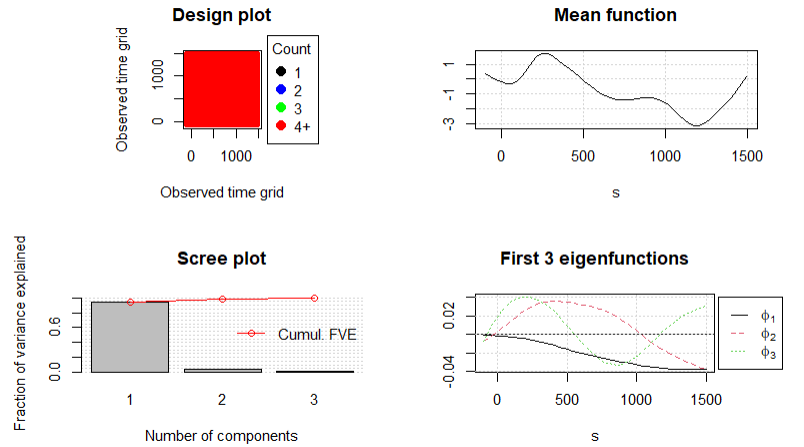
\includegraphics[width=0.8\linewidth]{Images/FPCA} 

}

\caption{FPCA visualisation - condition 1, trial 1}\label{fig:unnamed-chunk-3}
\end{figure}

As you can see the functional principal components are eigenfunctions
which explain the main modes of variation. We found we only needed three
functional principal components to explain 95\% of the variability in
the curves.

On the top right of this plot is the mean curve, and on the bottom
right, we can see the main modes of variation about this mean curve. So,
the mean curve is flattened to be a straight line, and the
eigenfunctions represent the functional principal components.

The first functional principal component, shown in black, remains close
to the mean function initially, and then it drops below the mean. In the
second FPC shown in red the eigenfunction rises above the mean and then
dropping below. The third initially rises above the mean then goes below
before rising above the mean again.

These are the three main ways in which subject's curves vary about the
mean and as we can see from the scree plot on the bottom left we can see
that the first FPC explains the most variance at approximately
\textasciitilde90\% and the second and third describe the remaining
\textasciitilde5\% of the variation.

\subsubsection{Investigating FPC scores}\label{investigating-fpc-scores}

To observe the principal component scores look like on our actual data,
we have plotted the subjects with the top and bottom scores for each
FPC.

\begin{figure}[H]

{\centering 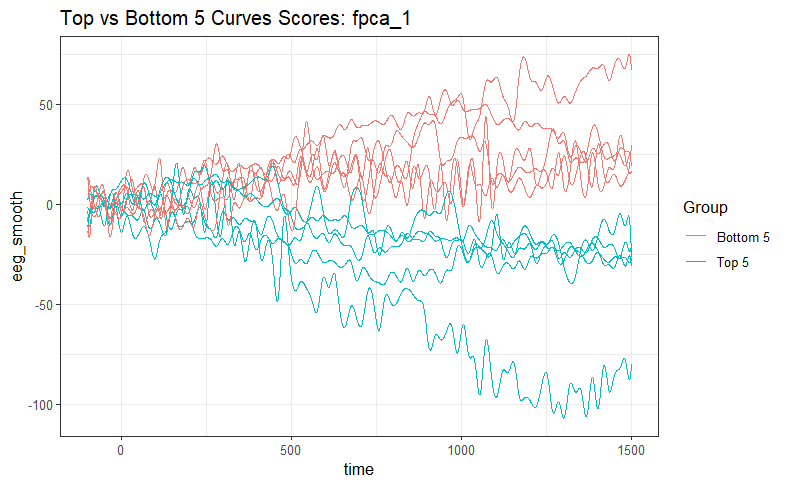
\includegraphics[width=0.8\linewidth]{Images/FPC1_top_bot} 

}

\caption{Curves with highest 5 FPC 1 scores (blue) and lowest 5 scores (red)}\label{fig:unnamed-chunk-4}
\end{figure}

\begin{figure}[H]

{\centering 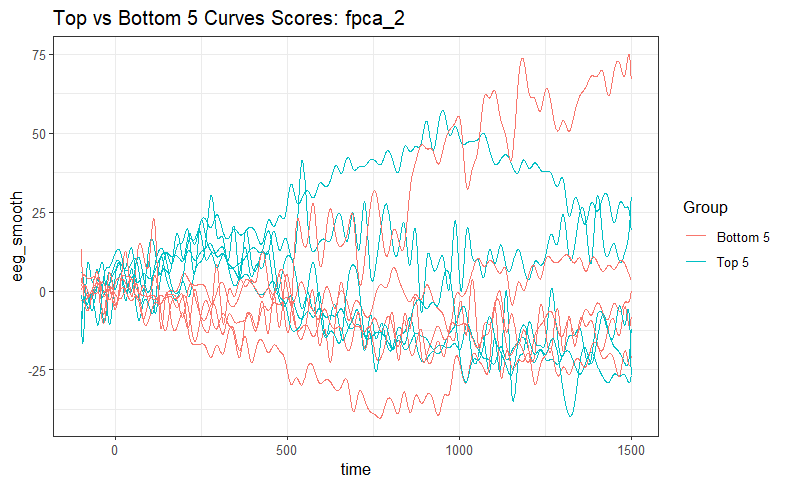
\includegraphics[width=0.7\linewidth]{Images/FPC2_top_bot} 

}

\caption{Curves with highest 5 FPC 2 scores (blue) and lowest 5 scores (red)}\label{fig:unnamed-chunk-5}
\end{figure}

\begin{figure}[H]

{\centering 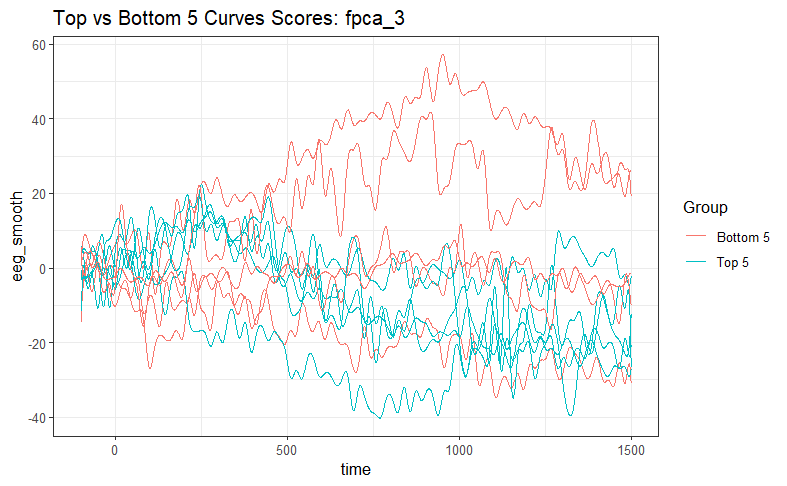
\includegraphics[width=0.7\linewidth]{Images/FPC3_top_bot} 

}

\caption{Curves with highest 5 FPC 3 scores (blue) and lowest 5 scores (red)}\label{fig:unnamed-chunk-6}
\end{figure}

\subsection{K-means clustering}\label{k-means-clustering}

\begin{figure}[H]

{\centering 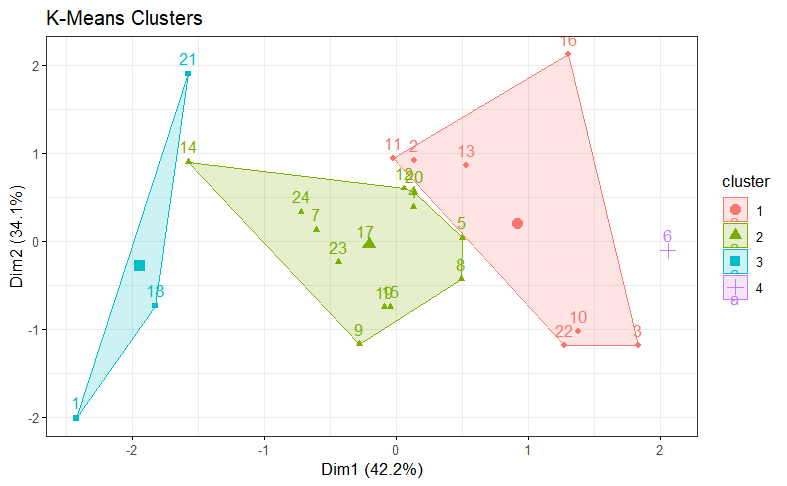
\includegraphics[width=0.7\linewidth]{Images/fpca_kmeans_plot} 

}

\caption{Visulisation of K-means clustering of FPC scores}\label{fig:unnamed-chunk-7}
\end{figure}

\begin{center}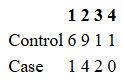
\includegraphics[width=0.12\linewidth]{Images/FPCA_km_cm} \end{center}

\begin{figure}[H]

{\centering 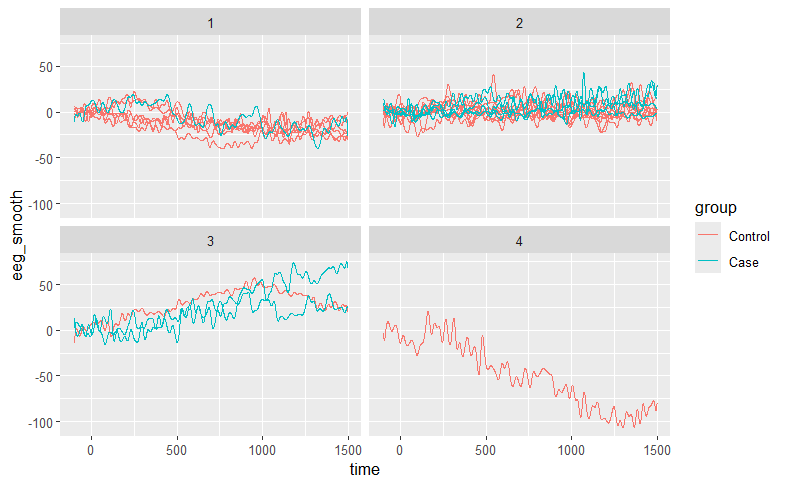
\includegraphics[width=0.7\linewidth]{Images/functions_by_cluster} 

}

\caption{Visulisation of functions in each of the K-means clusters}\label{fig:unnamed-chunk-9}
\end{figure}

\begin{itemize}
\tightlist
\item
  discuss FPCA components look like (top \& bottom 5 scores),
  eigenfunctions
\item
  discuss mfpca components - what do they look like
\item
  elastic net how many predictors included in final model
\end{itemize}

\section{Discussion}\label{discussion}

\label{sec:discussion}

\begin{itemize}
\tightlist
\item
  what does the permutation test tell us?
\item
  what di the fpcs tell us and what do the scores tell us about how much
  an individual eeg aligns with the eigenfunction?
\item
  what do the mfpcs tell us? at each level?
\item
  why do they differ at level 1? why is mfpca better/worse?
\item
  what can we conclude from elastic net - more less shrinkage? too few
  subjects?
\item
  How does our model perform - calibration curve, auc, misclassification
\item
  Anything that could further this research
\end{itemize}

\subsection*{References}\label{references}
\addcontentsline{toc}{subsection}{References}

\protect\phantomsection\label{refs}
\begin{CSLReferences}{1}{1}
\bibitem[\citeproctext]{ref-BOUTROS2009}
Boutros, Nash N., Anke Brockhaus-Dumke, Klevest Gjini, et al. 2009.
{``Sensory-Gating Deficit of the N100 Mid-Latency Auditory Evoked
Potential in Medicated Schizophrenia Patients.''} \emph{Schizophrenia
Research} 113 (2): 339--46.
https://doi.org/\url{https://doi.org/10.1016/j.schres.2009.05.019}.

\bibitem[\citeproctext]{ref-BugniHorowitz2021}
Bugni, Federico A., and Joel L. Horowitz. 2021. {``Permutation Tests for
Equality of Distributions of Functional Data.''} \emph{Journal of
Applied Econometrics} 36 (7): 861--77.

\bibitem[\citeproctext]{ref-BuiDing2025}
Bui, Lan N., and Qian Ding. 2025. {``Logistic Regression Modeling:
Methodological Insights and Roadmap.''} \emph{Currents in Pharmacy
Teaching and Learning} 17 (12): 102460.
\url{https://doi.org/10.1016/j.cptl.2025.102460}.

\bibitem[\citeproctext]{ref-Di2009}
Di, Chongzhi, Ciprian M. Crainiceanu, Brian S. Caffo, and Naresh M.
Punjabi. 2009. {``Multilevel Functional Principal Component Analysis.''}
\emph{The Annals of Applied Statistics} 3 (1): 458--88.
\url{https://doi.org/10.1214/08-AOAS206SUPP}.

\bibitem[\citeproctext]{ref-FortunaMaturo2019}
Fortuna, Fabio, and Francesca Maturo. 2019. {``K-Means Clustering of
Item Characteristic Curves and Item Information Curves via Functional
Principal Component Analysis.''} \emph{Quality \& Quantity} 53:
2291--304. \url{https://doi.org/10.1007/s11135-018-0724-7}.

\bibitem[\citeproctext]{ref-Gertheiss2024}
Gertheiss, Jan, David Rügamer, Bee Xian Wei Liew, and Sonja Greven.
2024. {``Functional Data Analysis: An Introduction and Recent
Developments.''} \emph{Biometrical Journal} 66 (6): e202300363.

\bibitem[\citeproctext]{ref-HoerlKennard1970}
Hoerl, Arthur E., and Robert W. Kennard. 1970. {``Ridge Regression:
Biased Estimation for Nonorthogonal Problems.''} \emph{Technometrics} 12
(1): 55--67. \url{https://doi.org/10.1080/00401706.1970.10488634}.

\bibitem[\citeproctext]{ref-JeonPolich2003}
Jeon, Yong-Wook, and John Polich. 2003. {``The P300 Event-Related
Potential in Psychosis: A Meta-Analysis.''} \emph{American Journal of
Psychiatry} 160 (10): 1789--98.

\bibitem[\citeproctext]{ref-RamsaySilverman2005}
Ramsay, James O., and Bernard W. Silverman. 2005. \emph{Functional Data
Analysis}. 2nd ed. Springer.

\bibitem[\citeproctext]{ref-SenkowskiGallinat2015}
Senkowski, Daniel, and Jürgen Gallinat. 2015. {``Dysfunctional
Prefrontal Gamma-Band Oscillations Reflect Working Memory and Other
Cognitive Deficits in Schizophrenia.''} \emph{Biological Psychiatry} 77
(12): 1010--19.

\bibitem[\citeproctext]{ref-Shen2020}
Shen, Chia-Ling, Tsung-Lin Chou, Wei-Shan Lai, et al. 2020. {``P50,
N100, and P200 Auditory Sensory Gating Deficits in Schizophrenia
Patients.''} \emph{Frontiers in Psychiatry} 11: 868.
\url{https://doi.org/10.3389/fpsyt.2020.00868}.

\bibitem[\citeproctext]{ref-Shin2011}
Shin, Yong-Wook, Jun Soo Kwon, Tae-Hoon Ha, et al. 2011. {``Gamma
Oscillation in Schizophrenia.''} \emph{Psychiatry Investigation} 8 (4):
288--96. \url{https://doi.org/10.4306/pi.2011.8.4.288}.

\bibitem[\citeproctext]{ref-Tibshirani1996}
Tibshirani, Robert. 1996. {``Regression Shrinkage and Selection via the
Lasso.''} \emph{Journal of the Royal Statistical Society: Series B
(Methodological)} 58 (1): 267--88.
\url{https://doi.org/10.1111/j.2517-6161.1996.tb02080.x}.

\bibitem[\citeproctext]{ref-ZouHastie2005}
Zou, Hui, and Trevor Hastie. 2005. {``Regularization and Variable
Selection via the Elastic Net.''} \emph{Journal of the Royal Statistical
Society: Series B (Statistical Methodology)} 67 (2): 301--20.
\url{https://doi.org/10.1111/j.1467-9868.2005.00503.x}.

\end{CSLReferences}

\bibliographystyle{unsrt}
\bibliography{references.bib}


\end{document}
